\subsection*{Navneordsanalyse (Martin)}
\addcontentsline{toc}{subsection}{Navneordsanalyse}
Udfra use casene har vi beskrevet vores problemstillinger:\\
En rekvirent logger ind og sender en rekvisition og evt. et kontrolskema. Disse
indeholder data om en patient, og om hvilken slags undersøgelse, der ønskes,
samt prioritet og ønsket dato af undersøgelsen. Brugeren kan annullere en
rekvisition.\\
En visitator logger ind og henter en liste over rekvisitioner. Visitatoren
vælger en rekvisition og gennemgår de relevante info. Alt efter om rekvisitionen
er i orden godkender eller afviser han den.\\
En sekretær logger ind og henter en liste over rekvisitioner, der skal bookes.
Sekretæren booker tider ved det nødvendige udstyr til hver undersøgelse og
sender notifikationer til alle interessenter.\\
En administrator logger ind og kan enten ændre rettigheder for en bruger,
oprette en bruger eller slette en bruger.”\\
Herfra finder vi de relevante navneord, dem der umiddelbart ikke bare skal være
en attribut, og opstiller en liste, med de relevante udsagnsord efter. Navneord
bliver ofte til klasser i et program, og udsagnsord bliver ofte til metoder
øvrige navneord/tillægsord bliver ofte til attributter. Vi har markeret
udsagnsord der forventes at blive til metoder med kursiv.
\textbf{Rekvirent} - \emph{send rekvisition} og evt. et kontrolskema, 
\emph{annuller rekvisition}\\
\textbf{Patient} - tilknyttet rekvisition og patient data\\
\textbf{Rekvisition/Kontrolskema} - indeholder data om patient, hvilken slags
undersøgelse ønskes, prioritet og ønsket dato af undersøgelse\\
\textbf{Visitator} - \emph{log ind}, \emph{se liste over rekvisitioner},
\emph{vælg rekvisition}, \emph{godkend rekvisition}, afvis 
\textbf{Rekvisition} - sendes af rekvirent, modtages af visitator og sekretær,
visiteres, stemples godkendt eller afvist\\
\textbf{Sekretær} - \emph{log ind}, \emph{se liste} over rekvisitioner, marker
rekvisition som læst, \emph{book} tider/udstyr, \emph{send notifikationer} til
interessenter\\
\textbf{Undersøgelse} - tidspunkt, type\\
\textbf{Notifikation} - sendes til interessenter af sekretær\\
\textbf{Interessenter} - modtager notifikation\\ 
\textbf{Administrator} - \emph{log ind}, \emph{ændre rettigheder for bruger},
\emph{opret bruger}, \emph{slet bruger}\\
\textbf{Bruger} - liste af rettigheder
\FloatBarrier
\begin{figure}[h]
\subsection*{CRC-kort (Rúni, Morten)}
\addcontentsline{toc}{subsection}{CRC-kort}
\centering
\makebox[\textwidth]{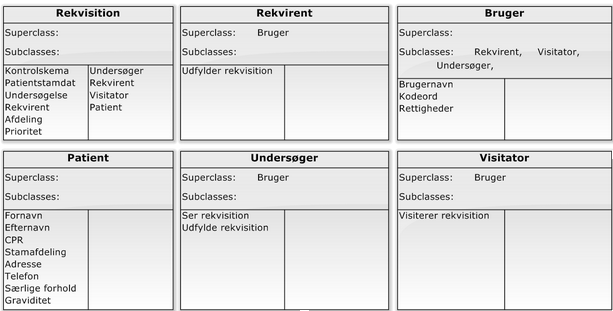
\includegraphics[width=\textwidth]{CRC}}
\caption{\emph{CRC diagram}: Viser de overordnede relationer projektet
indeholder. \label{crc_kort}}
\end{figure}
\FloatBarrier
\subsection*{Domænemodel (Rúni, Magnus)}
\addcontentsline{toc}{subsection}{Domænemodel}
Vi har løbende opdateret vores domænemodel (se original model i
\hyperref[Bilag17]{bilag 17}) til at afspejle den del af rekvisitionssystemet vi
vil arbejde med (\hyperref[domainmodel]{figur \ref*{domainmodel}}).
Rekvirenten, visitatoren og sekretæren er brugere på vores system, hvor de har
mulighed for at udføre deres opgaver.
\FloatBarrier
\begin{figure}[h]
\centering
\makebox[\textwidth]{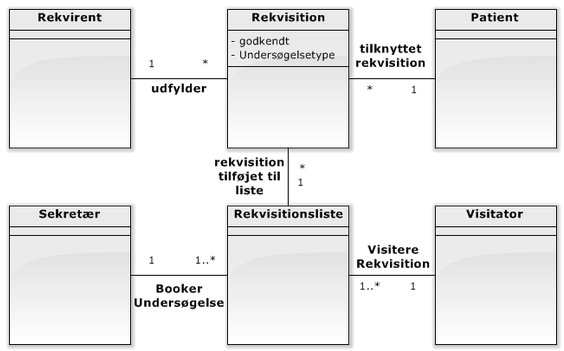
\includegraphics[width=\textwidth]{Domainmodel}}
\caption{\emph{Domænemodel}: \label{domainmodel}}
\end{figure}
\FloatBarrier
\begin{figure}[h]
\subsection*{System sekvens diagram (Morten)}
\addcontentsline{toc}{subsection}{System sekvens diagram}
\centering
\makebox[\textwidth]{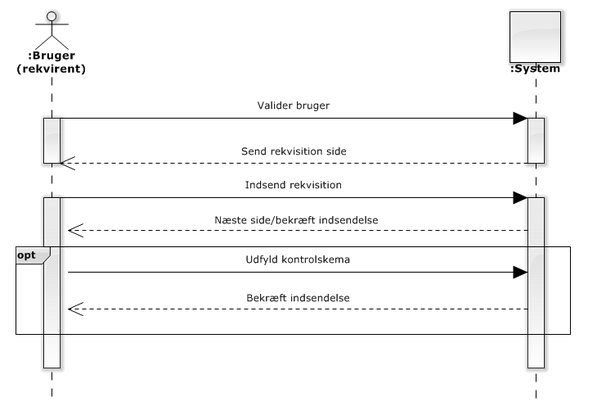
\includegraphics[width=\textwidth]{SSD1}}
\caption{\emph{SSD} over use casen “bestil undersøgelse”. Når brugeren har
udfyldt rekvisitionen, kan der til nogle undersøgelsestyper være et tilknyttet
et kontrolskema som også skal udfyldes. \label{ssd_1}}
\end{figure}
Yderligere et SSD over use casen visiter rekvisition ses i
\hyperref[Bilag18]{bilag 18}.
\FloatBarrier
\subsection*{Database Analyse (Christian, Magnus)}
\addcontentsline{toc}{subsection}{Database Analyse}
Vi startede med at analysere hele arbejdsgangen, og de data, der bruges til at
holde styr på rekvisition/undersøgelser som en skitse af et E/R diagram (se
\hyperref[Bilag19]{bilag 19}). Det gav os et meget stort E/R diagram, der ikke
ville kunne implementeres på en rimelig tid.\\
Efter vores møde og interview med interessenterne skar vi vores arbejdsområde
ned til selve rekvisitionen af en billeddannende undersøgelse.
\FloatBarrier
\begin{figure}[h]
\centering
\makebox[\textwidth]{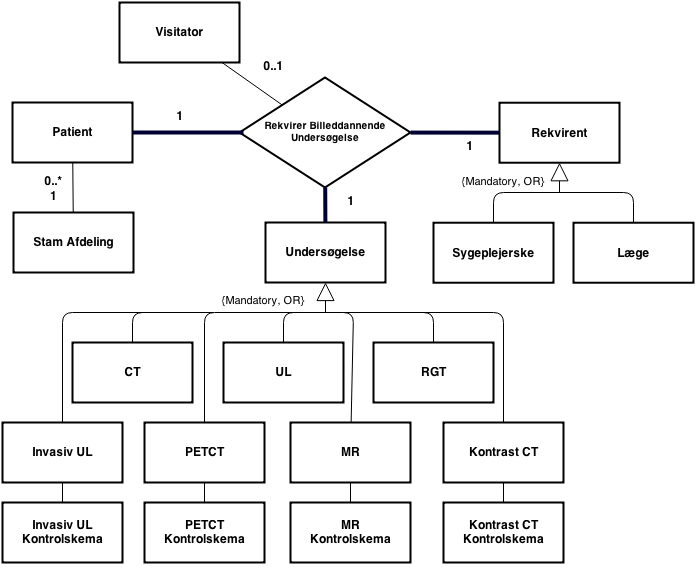
\includegraphics[width=\textwidth]{E-R_Diagram}}
\caption{\emph{E/R diagram}. Beskriver sammenhæng mellem entiteterne. Vi har en
central relation - selve rekvisitionen, tegnet som en rhombe. Rekvirent, Patient
og Undersøgelse er alle obligatoriske i relationen, hvorimod en visitator
tilknyttes senere. Rekvirenten modelleres senere som en tabel
(sygeplejerske/læge distinktionen udgår). Stamafdelingen reduceres til en
attribut. \label{er_diagram}}
\end{figure}
\FloatBarrier